\section{Modi normali della struttura solare}

\begin{frame}[label=noinside]{Modi di oscillazione adiabatici}{Perturbazione dello stato di equilibrio.}

\begin{block}{campi di velocit\'a/effetti non lineari}
Descrivo le oscillazioni come piccole perturbazioni attorno allo stato di equilibrio stazionario (gli effetti non lineari, fra cui lo scambio di energia tra i modi, sono dell'ordine di $\frac{v}{c_s}$ dove v \'e l'ampiezza della velocit\'a dell'oscillazione). 
In generale pu\'o essere presente un campo di velocit\'a $\vec{v}_0$:
\begin{align}
&\vec{v}=\vec{v}_0+\vec{v}'\\
&\TDof{t}=\PDof{t}+(\vec{v}_0\cdot\nabla)
\end{align}
in prima approssimazione prendo $\vec{v}_0=0$ per poi considerare come perturbazioni gli effetti dovuti a campi di velocit\'a in specie rotazione.

\end{block}

\begin{block}{Perturbazione pressione densit\'a}

Indico con $P'(\vec{r},t)$ e $\delta P$ la perturbazione euleriana e lagrangiana della pressione e con $\rho'$, $\Phi'$ e $\vec{g}'$ la perturbazione euleriana della densit\'a , e le perturbazioni euleriane del potenziale gravitazionale e dell'accelerazione di gravit\'a conseguenti  con $\delta\vec{r}=\vec{\xi}$ il vettore spostamento perturbato:
\begin{align}
&P(\vec{r},t)=P_0(\vec{r})+P'(\vec{r},t)\label{eq:pressureperturbation}\\
&\Lvar{P(\vec{r})}=P(\vec{r}+\Lvar{\vec{r}})-P_0(\vec{r})=P'(\vec{r})+\Lvar{\vec{r}}\cdot\nabla P_0\\
&\vec{g}'=-\nabla\Phi',\ \nabla^2\Phi'=4\pi G\rho'\label{eq:gapert}
\end{align}

\end{block}


\end{frame}

\begin{frame}[label=noinside]{Modi di oscillazione adiabatici}{Modi di oscillazione lineari adiabatici.}

\begin{block}{Equazione del moto perturbata}

l'equazione del moto perturbato sostituendo \eqref{eq:pressureperturbation} nell'equazione del moto \eqref{eq:motion} considerando solo i termini lineari nella perturbazione:
\begin{equation}
\rho_0\TDof{t}\vec{v}=\rho_0\PtwoDy{t}{\Lvar{\vec{r}}}=-\nabla P'+\rho_0\vec{g}'+\rho'\vec{g}_0\label{eq:emper}
\end{equation}

\end{block}

\end{frame}

\begin{frame}[label=noinside]{Modi di oscillazione adiabatici}{Equazione di continuit\'a perturbata}

\begin{block}{Equazione di continuit\'a perturbata}

Analogamente per l'equazione di continuit\'a ottengo
\begin{equation}
\rho'+\div{(\rho_0\Lvar{\vec{r}})}=0\label{eq:contper}
\end{equation}

\end{block}

\end{frame}

\begin{frame}[label=noinside]{Modi di oscillazione adiabatici}{Condizione di adiabaticit\'a}


  \begin{overlayarea}{\textwidth}{1cm}
   \only<1>{
   energia interna per unit\'a di massa
\begin{equation}
\TDy{t}{q}=\TDy{t}{u}+P\TDof{t}(\frac{1}{\rho})\label{eq:prima}
\end{equation}

\begin{equation}
\TDy{t}{T}-\frac{\Gamma_2-1}{\Gamma_2}\frac{T}{P}\TDy{t}{P}=\frac{1}{c_P}(\epsilon-\frac{1}{\rho}\scap{\nabla}{F})
\end{equation}
il termine a destra \'e trascurabile:
\begin{equation}
\TDy{t}{q}=0
\end{equation}
   }
   \only<2>{
   Il moto di una elemento di fluido \'e descritto dalla relazione adiabatica
\begin{equation}
\TDy{t}{P}=\frac{\Gamma_1P}{\rho}\TDy{t}{\rho}
\end{equation}
}
   \only<3>{
  
  La condizione di perturbazione adiabatica linearizzata \'e
\begin{align}
&\PDy{t}{\Lvar{P}}-\frac{\Gamma_{1,0}P_0}{\rho_0}\PDy{t}{\Lvar{\rho}}=0\\
&P'+\Lvar{\vec{\xi}}\cdot\nabla P_0=\frac{\Gamma_{1,0}P_0}{\rho}(\rho'+\Lvar{\vec{\xi}}\cdot\nabla\rho_0)\label{eq:adper}
\end{align}

   }
  \end{overlayarea}


\end{frame}


\begin{figure}[!ht]

\subfigure[Distribuzione dei modi con $l\leq300$ nel diagramma $\nu-l$ determinata usando i primi 144 giorni di osservazione di MDI. Da \cite{chr02helioseismology}.]{
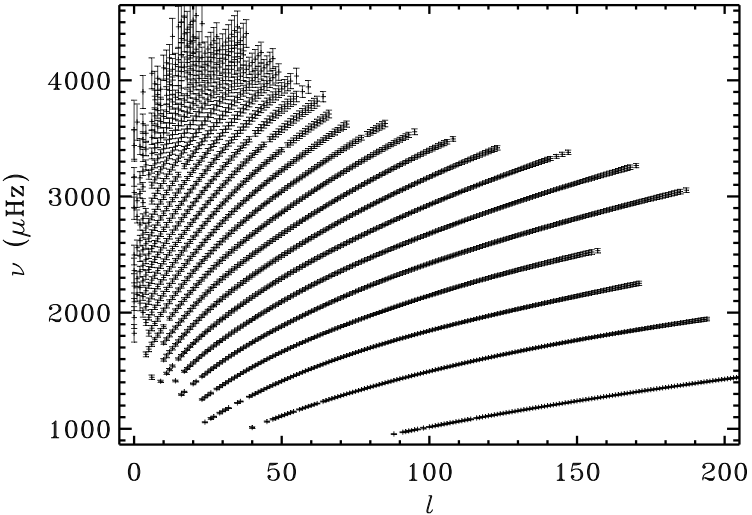
\includegraphics[keepaspectratio,width=0.45\textwidth]{midlmodes}}
\label{fig:midlmodes}
~
\subfigure[Modi adiabatici calcolati sulla base di un modello solare. Da \cite{chr02helioseismology}.]{
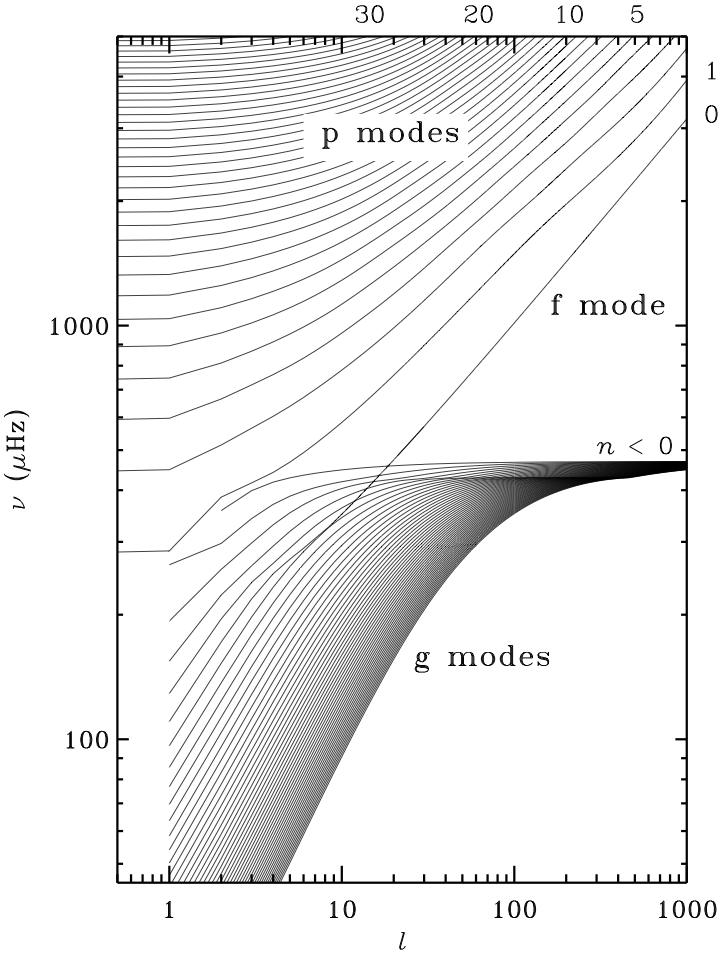
\includegraphics[keepaspectratio,width=0.6\textwidth]{nrmodesLAWE}\label{fig:nrmodesLAWE}}

\end{figure}

%%% SOS

\begin{frame}{Oscillazioni dei 5 minuti}

\begin{block}{Comportamento periodico dell'atmosfera solare con grande coerenza spaziale e temporale}

In \citet{lei62velocity} si osserva che la superficie solare ha scale spazio-temporali privilegiate: in particolare \'e presente un comportamento periodico nell'atmosfera a tutte le altezze rilevato tramite effetto doppler. Il periodo \'e di circa 300 secondi e la lunghezza caratteristica di qualche \si{\mega\meter}.

\end{block}

\begin{block}{Modi normali - onde gravo-acustiche in cavit\'a risonanti di varia profondit\'a}

Il modello proposto da \citet{ulrich70five} e \citet*{stein71five} considera le propriet\'a dei modi normali non radiali di oscillazione del Sole, in particolare usando la relazione di dispersione per onde acustiche, si ha la definizione di cavit\'a risonanti all'interno del Sole: la variazione delle propriet\'a del gas delimita le regioni di propagazione a diverse profondit\'a a seconda delle caratteristiche trasversali del moto.

\end{block}

\end{frame}

\subsection{Perturbazione adiabatiche.}

\begin{frame}{Perturbazioni adiabatiche}


con $\vec{v}'$ perturbazione euleriana della velocit\'a. La variazione di una grandezza euleriana nel riferimento solidale con l'elemento di fluido si esprime tramite
\begin{align}
&\vec{v}=\vec{v}_0+\vec{v}'
&\TDof{t}=\PDof{t}+(\vec{v}_0\cdot\nabla)
\end{align}

\begin{align}
&P(\vec{r},t)=P_0(\vec{r})+P'(\vec{r},t)\label{eq:pressureperturbation}\\
&\Lvar{P(\vec{r})}=P(\vec{r}+\Lvar{\vec{r}})-P_0(\vec{r})=P'(\vec{r})+\Lvar{\vec{r}}\cdot\nabla P_0\\
&\vec{g}'=-\nabla\Phi',\ \nabla^2\Phi'=4\pi G\rho'\label{eq:gapert}
\end{align}
Ricavo l'equazione del moto perturbato sostituendo \eqref{eq:pressureperturbation} nell'equazione del moto \eqref{eq:motion} considerando solo i termini lineari nella perturbazione:
\begin{equation}
\rho_0\TDof{t}\vec{v}=\rho_0\PtwoDy{t}{\Lvar{\vec{r}}}=-\nabla P'+\rho_0\vec{g}'+\rho'\vec{g}_0\label{eq:emper}
\end{equation}

Analogamente per l'equazione di continuit\'a ottengo
\begin{equation}
\rho'+\div{(\rho_0\Lvar{\vec{r}})}=0\label{eq:contper}
\end{equation}

L'equazione di conservazione dell'energia interna \eqref{eq:primatemp}, esplicitando il bilancio di calore \eqref{eq:heatgl}, \'e

\begin{equation}
\TDy{t}{T}-\frac{\Gamma_2-1}{\Gamma_2}\frac{T}{P}\TDy{t}{P}=\frac{1}{c_P}(\epsilon-\frac{1}{\rho}\scap{\nabla}{F})
\end{equation}

Mostro schematicamente che il termine a destra \'e trascurabile su tempi del periodo delle oscillazioni solari.

Entrambi i tempi scala per scambio di calore sono molto maggiori del periodo delle oscillazioni quindi su un periodo i termini dovuti allo scambio di calore sono trascurabili; l'approssimazione adiabatica non \'e pi\'u valida vicino alla superficie solare dove i tempi per lo scambio di calore sono pi\'u brevi.

Il moto di una elemento di fluido \'e descritto dalla relazione adiabatica
\begin{equation}
\TDy{t}{P}=\frac{\Gamma_1P}{\rho}\TDy{t}{\rho}
\end{equation}

La condizione di perturbazione adiabatica linearizzata \'e:
\begin{align}
&\PDy{t}{\Lvar{P}}-\frac{\Gamma_{1,0}P_0}{\rho_0}\PDy{t}{\Lvar{\rho}}=0\intxt{che integrata rispetto a t ed in funzione della variazione euleriana diventa}
&P'+\vec{\xi}\cdot\nabla P_0=\frac{\Gamma_{1,0}P_0}{\rho}(\rho'+\vec{\xi}\cdot\nabla\rho_0)\label{eq:adper}
\end{align}

Cerco una soluzione della forma di un'onda stazionaria: esprimo la dipendenza temporale tramite $\exp{i\omega t}$ e angolare tramite le funzioni armoniche sferiche $Y_{lm}(\theta,\phi)$ con:
\begin{align}
&Y_{lm}(\theta,\phi)=(-)^mc_{lm}P_l^m(\cos{\theta})\exp{im\phi}\\
&L^2Y_l^m=-\frac{1}{\sin{\theta}}\PDof{\theta}(\sin{\theta}\PDy{\theta}{Y_l^m})+\frac{1}{\sin^2{\theta}}\PtwoDy{\phi}{Y_l^m}=-r^2\nabla_h^2Y_l^m=l(l+1)Y_l^m\label{eq:SHperturb}
\end{align}
e scrivo la variazione euleriana di densit\'a, pressione e potenziale gravitazionale nella forma
\begin{equation}
(\rho',P',\Phi')=\exp{i\omega t}[\rho'(r),P'(r),\Phi'(r)]Y_l^m
\end{equation}

\end{frame}

\begin{frame}{Frequenze e autofunzioni del vettore perturbato}


Dall'equazione del moto \eqref{eq:emper}, poich\'e le deviazioni dalla simmetria sferica sono in prima approssimazione trascurabili, \'e evidente che:
\begin{equation}
%&\omega^2\vec{\xi}=\nabla a+\frac{N^2c^2}{g}b\frac{\vec{r}}{r}\\
\hat{r}\cdot(\rot{\vec{\xi}})=0\ \Rightarrow\ \PDof{\theta}(\sin{\theta}\xi_{\phi})-\PDy{\phi}{\xi_{\theta}}=0
\end{equation}
ed \'e quindi possibile ricavare la componente tangenziale della perturbazione da una funzione scalare:
\begin{equation}
\vec{\xi}=\exp{i\omega t}(\xi_r(r),\xi_h(r)\PDof{\theta},\frac{\xi_h(r)}{\sin{\theta}}\PDof{\phi})Y_l^m(\theta,\phi)
\end{equation}
dove ho scomposto il vettore spostamento perturbato in componente radiale $\xi_r(r)$ e tangenziale $\xi_h(r)$.

Ricavo la componente $\xi_h(r)$ applicando la parte tangenziale della divergenza all'equazione del moto:
\begin{equation}
\xi_h(r)=\frac{L}{r\omega^2}(\frac{P'(r)}{\rho_0}+\Phi'(r))
\end{equation}
infine $\xi_r(r)$, $P'(r)$ e $\Phi'(r)$ sono determinati da
\begin{subequations}\label{eigenomega}
\begin{align}
&\frac{1}{r^2}\TDof{r}(r^2\xi_r)-\frac{\xi_rg}{c^2}+\frac{1}{\rho_0}(\frac{1}{c^2}-\frac{l(l+1)}{r^2\omega^2})P'-\frac{l(l+1)}{r^2\omega^2}\Phi'=0\\
&\frac{1}{\rho_0}(\TDof{r}+\frac{g}{c^2})P'-(\omega^2-N^2)\xi_r+\TDy{r}{\Phi'}=0\\
&\frac{1}{r^2}\TDof{r}(r^2\TDy{r}{\Phi'})-\frac{l(l+1)}{r^2}\Phi'-\frac{4\pi G\rho_0}{g}N^2\xi_r-\frac{4\pi G}{c^2}P'=0
\end{align}
\end{subequations}
con $g=-\frac{1}{\rho_0}\TDy{r}{P_0}$.

Il sistema di equazione \eqref{eigenomega} ha soluzione con le opportune condizioni al contorno per un insieme discreto di valori delle frequenze, $\omega_{nlm}$. L'ordine angolare m non compare nelle equazioni quindi gli autovalori $\omega_{nlm}$ sono $2l+1$ degeneri: la degenerazione \'e rimossa nel caso si tenga conto della rotazione ($\frac{\Omega}{\omega}\approx\num{e-4}$).
%o di effetti gravitazionali di altri corpi.

Condizioni al contorno: sono necessarie 4 condizioni.
\begin{itemize}
\item Due condizioni per $r=0$ selezionano le soluzioni regolari:
\begin{equation}
P'=0,\ \Phi'=0
\end{equation}
Vicino a zero risulta un andamento asintotico
\begin{equation}
(l\neq0):\ \xi_r\propto r\expy{l-1};\ (l=0):\ \xi_r\propto r;P',\ \Phi'\propto r^l
\end{equation}

\item Alla superficie solare richiediamo la continuit\'a di $\Lvar{\nabla\Phi}$ e che non si abbia propagazione verso l'esterno.
All'esterno della stella ho $\rho'=0$ quindi scelgo la soluzione nulla a infinito dell'equazione di Poisson $\Phi'=Ar\expy{-l-1}$:
\begin{equation}
\TDy{r}{\Phi'}+\frac{l+1}{r}\Phi'=0,\ r=\rsun{}    
\end{equation}
La condizione di non propagazione oltre la fotosfera dipende dalla descrizione dell'atmosfera solare. Nella versione pi\'u semplice impongo che la variazione di pressione sia zero alla superficie perturbata della stella
\begin{align}
&\Lvar{P}=P'+\xi_r\TDy{r}{P}=0
\end{align}
\end{itemize}

\end{frame}

\begin{frame}{Diagramma $\nu-l$ per i modi adiabatici}

\begin{figure}[!ht]
\subfigure[I picchi della densit\'a spettrale si dispongono su creste in cui \'e concentrata la potenza in accordo al modello. Determinata usando i primi 144 giorni di osservazione di MDI con $l\leq300$. Da \cite{chr02helioseismology}.]{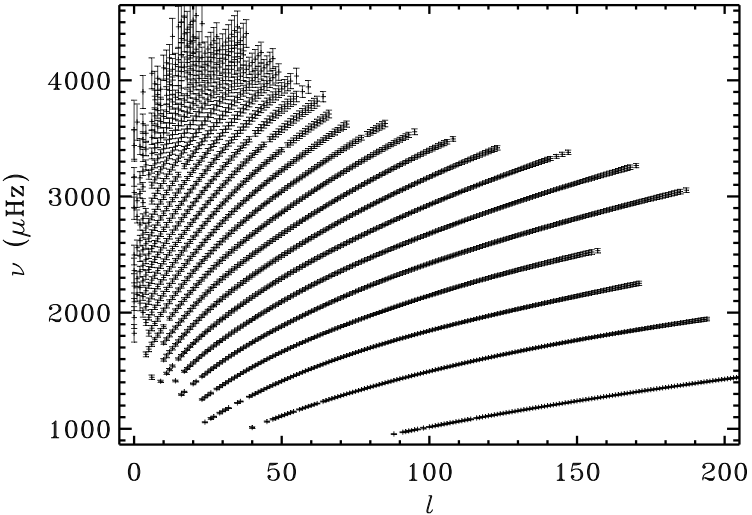
\includegraphics[keepaspectratio,width=0.45\textwidth]{midlmodes}}
\label{fig:midlmodes}
~
\subfigure[Modi adiabatici calcolati sulla base di un modello solare. Da \cite{chr02helioseismology}.]{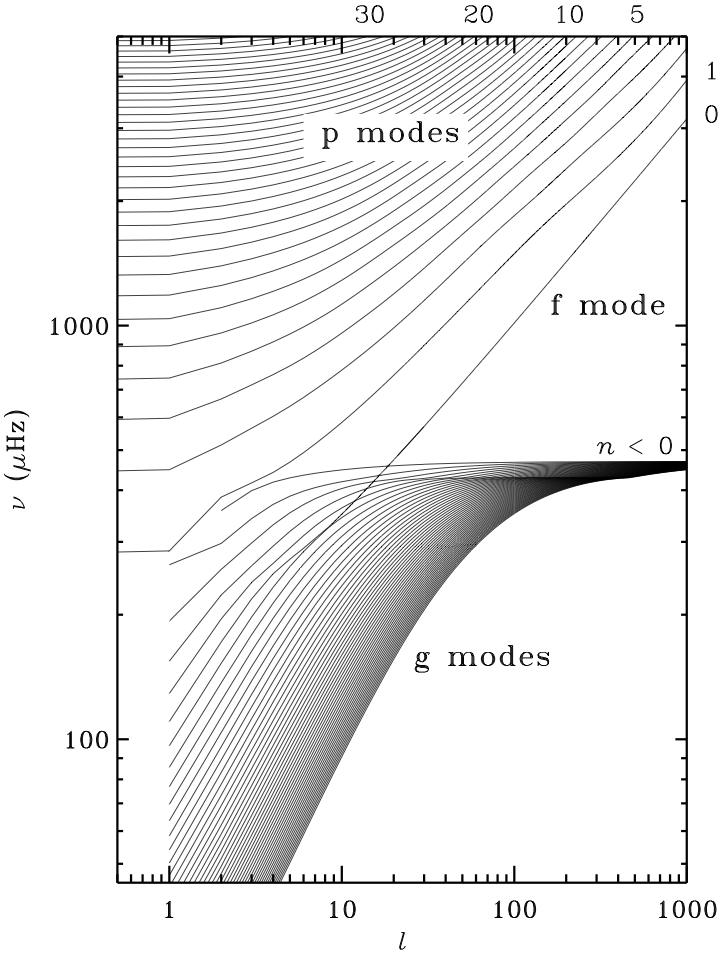
\includegraphics[keepaspectratio,width=0.95\textwidth]{nrmodesLAWE}}
\label{fig:nrmodesLAWE}

\end{figure}

\end{frame}

\subsection{Energia dei modi-effetti di superficie}

Indico con $\exv{E_{kin}^{nl}}$ la media temporale dell'energia cinetica del modo
\begin{equation}
E_{kin}^{nl}=\frac{1}{2}\int_V|\vec{v}|^2\rho_0\,dV=\frac{\omega^2}{2}\int_V|\vec{\xi}|^2\rho_0\,dV
\end{equation}
cio\'e
\begin{equation}
\exv{E_{kin}^{nl}}=\frac{1}{\Pi}\int_0^{\Pi}E_{kin}^{nl}=\frac{1}{2}I_{nl}\exv{\dvec{\xi}_{nl}(R)}^2
\end{equation}
dove $\exv{\dvec{\xi}_{nl}(R)}$ indica la velocit\'a quadratica media superficiale e ho definito l'inerzia normalizzata:
\begin{equation}\label{eq:normalizedinertia}
I_{nl}=\frac{1}{M\exv{\vec{\xi}(R)\vec{\xi}^*(R)}}\int_V\,d^3x\rho_0\vec{\xi}\vec{\xi}^*
\end{equation}

Le oscillazioni solari sono in prevalenza dovute ad onde acustiche, in cui la forza di richiamo \'e prodotta dal gradiente di pressione, modi p, e onde in cui la forza di richiamo \'e la forza di gravit\'a, i modi g: i modi osservabili pi\'u facilmente hanno periodo attorno a \SI{5}{\minute} ci\'o \'e dovuto all'aumento del rumore solare a basse frequenze e ai processi di eccitazione dei modi che trasferiscono la massima energia ai modi di tale periodo.

\begin{figure}[!ht]

\begin{subfigure}[b]{0.45\textwidth}
\centering
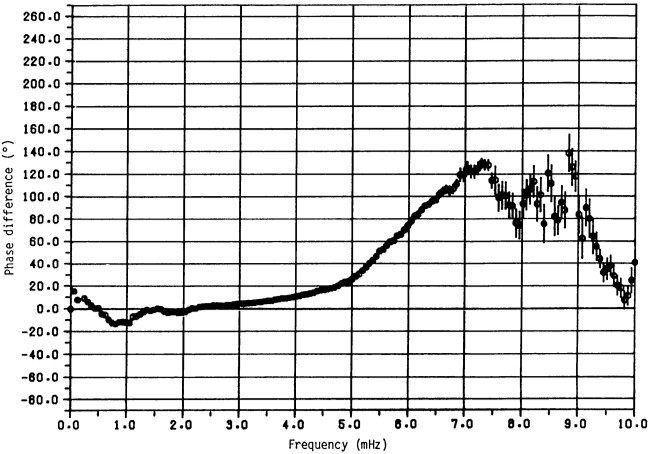
\includegraphics[keepaspectratio,width=0.9\textwidth]{phasepropagation}
\caption{Differenza di fase per il segnale Doppler delle righe $(5930)$ Fe I, pi\'u profonda, e $(5896)$ Na I, pi\'u alta nell'atmosfera. Da \cite{staiger1987observations}.}\label{fig:phasedifference}
\end{subfigure}
~
\begin{subfigure}[b]{0.45\textwidth}
\centering
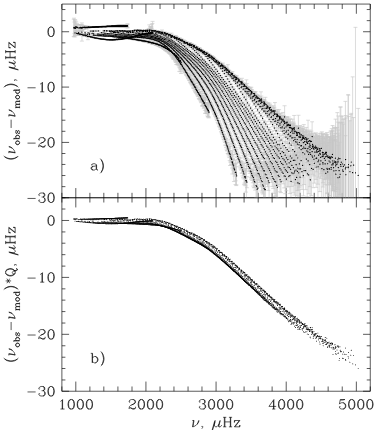
\includegraphics[keepaspectratio,width=0.9\textwidth]{domega}
\caption{In alto: differenze tra frequenze dei modi teoriche e osservate. In basso: differenze moltiplicata per $Q_{nl}$: viene rimossa la dipendenza da l dovuta alla maggiore ampiezza delle autofunzioni nelle regioni superficiali in cui l'approssimazione adiabatica non \'e corretta. Da \cite{rhodesmeasurements}.}\label{fig:nFreqdiff}
\end{subfigure}

\end{figure}

Nella figura (\subref{fig:nrmodesLAWE}) sono mostrate le frequenze dei modi soluzioni del sistema \eqref{eigenomega} calcolati usando le grandezze di equilibrio di un modello solare, in (\subref{fig:midlmodes}) le frequenze misurate e in \subref{fig:nFreqdiff} le differenze tra frequenze predette e osservate.

Gli effetti dovuti alla non corretta descrizione fisica dei modi vicino alla superficie, $r>0.95\rsun{}$ sono maggiori per i modi di l elevato perch\'e confinati in gusci meno profondi al crescere di l. Introduco il rapporto d'inerzia:
\begin{align}
%&\frac{V_{nl}}{V_0(\nu_{nl})}=(Q_{nl})\expy{-\midfrac{1}{2}}\intxt{dove ho introdotto l'inerzia e il rapporto d'inerzia $Q_{nl}$}
&Q_{nl}=\frac{I_{nl}}{I^0_{nl}}\label{eq:surfaceeffects}
\end{align}
$Q_{nl}=1$ per $l=0$ e diminuisce al crescere di $l$; l'ampiezza superficiale relativa al modo radiale estrapolato a frequenza $\nu_{nl}$, $\frac{A_{nl}(\nu_{nl})}{A_{nl}^0(\nu_{nl})}\propto(Q_{nl})\expy{-\midfrac{1}{2}}$, cresce con l.

Il comportamento all'aumentare della frequenza mostrato in \subref{fig:nFreqdiff} \'e dovuto al fatto che per frequenze maggiori la regione in cui si ha riflessione interna \'e pi\'u in alto dove l'approssimazione adiabatica \'e meno valida; la figura \subref{fig:phasedifference} mostra la propagazione di fase ad alte frequenze dovuta ad effetti dissipativi.


\subsection{Principio variazionale}    %Vedi pg 110 dalsnote.

\begin{frame}{Variazioni nel modello provocano variazioni nelle frequenze dei modi}

EOM lionearizzata

\begin{equation}\label{eq:EOMrhoc}%Unno89
-\omega^2\rho_0\xi=\nabla(c_s^2\rho\scap{\nabla}{\xi}+\nabla P\cdot\vec{\xi})-\vec{g}_0\nabla\cdot(\rho_0\vec{\xi})-G\rho_0\nabla(\int_V\frac{\nabla\cdot(\rho_0\vec{\xi})\,d^3r'}{|\vec{r}-\vec{r}'|})
\end{equation}

\citet{Cha64Variational} ha dimostrato che questo costituisce un problema agli autovalori hermitiano per condizioni ai bordi di pressione e densit\'a nulle quindi $\omega^2$ \'e reale e autofunzioni di frequenza caratteristica diversa sono ortogonali:
\begin{equation}
\int\vec{\xi}_i*\vec{\xi}_j\rho\,d^3x=0
\end{equation}

\'E utile scrivere la relazione tra variazioni nell'operatore lineare $L$ e differenze nelle frequenze caratteristiche:
\begin{equation}
(L+\Lvar{L})(\xi+\Lvar{\xi})=-(\omega+\Lvar{\omega})^2(\xi+\Lvar{\xi})\label{eq:EMvar}
\end{equation}
quindi considerando i termini lineari nelle variazioni e dato che le frequenze caratteristiche sono stazionarie per variazioni di $\xi$ si ha la relazione:
\begin{equation}\label{eq:variational}
\frac{\Lvar{\omega}}{\omega}=-\frac{\int_V\rho\vec{\xi}\Lvar{L}\vec{\xi}\,d^3x}{2\omega^2\int_V\rho\scap{\xi}{\xi}d^3x}
\end{equation}

\end{frame}

\subsection{Variazioni struttura idrostatica e variazioni nell'equazione di stato e nella  composizione}

\begin{frame}{Variazioni struttura idrostatica}

Esplicito la forma della perturbazione $\delta L$ in \eqref{eq:EOMrhoc} introducendo piccole variazioni nel profilo di $\rho$ e $c_s$:
\begin{equation}
\Lvar{L}\vec{\xi}=\nabla(\Lvar{c_s^2}\nabla\cdot\vec{\xi}+\Lvar{\vec{g}}\cdot\vec{
\xi})+\nabla(\frac{\Lvar{\rho}}{\rho_0})c^2\nabla\cdot\vec{\xi}+\frac{1}
{\rho_0}\nabla\rho_0\Lvar{c_s^2}\nabla\vec{\xi}+\Lvar{\vec{g}}\nabla\cdot\vec{\xi}-
G\nabla\int_V\frac{\nabla\cdot(\Lvar{\rho}\xi)}{|\vec{x}-
\vec{x}'|}\,d^3x'\label{eq:eqmotvar}
\end{equation}
con
\begin{equation}
\Lvar{g}(r)=\frac{4\pi G}{r^2}\int_0^r\Lvar{\rho}(s)s^2\,ds
\end{equation}

\'E quindi possibile esprimere le differenze nelle frequenze dei modi nella forma
\begin{equation}\label{eq:hydroefdiff}
\frac{\delta\omega_{nl}}{\omega_{nl}}=\int_0^R[K^{nl}_{c^2,\rho}(r)\frac{\delta_rc^2}{c^2}(r)+K^{nl}_{\rho,c^2}(r)\frac{\delta_r\rho}{\rho}(r)]\,dr+I_{nl}\expy{-1}F_{Surf}
\end{equation}

I kernel $K_Q^j$ dipendono dalle autofunzioni del modello solare, il termine $I_{nl}\expy{-1}F_{Surf}(\omega_{nl})$ tiene conto degli effetti superficiali.

\begin{equation}
\Lvar{P}=\int_r^R(g\Lvar{\rho}+\rho\Lvar{g})\,dr\label{eq:pressurecorrho}
\end{equation}

\end{frame}

\begin{frame}{Variazioni equazione di stato e composizione}

Dipendenza di $\Gamma_1(P,\rho,X_i)$ dalla composizioneriscrivendo \eqref{eq:hydroefdiff} nella forma:
\begin{align}
&\frac{\delta\omega_{nl}}{\omega_{nl}}=\int_0^R[K^{nl}_{\Gamma_1,\rho}(r)\frac{\delta_r\Gamma_1}{\Gamma_1}(r)+K^{nl}_{\rho,\Gamma_1}(r)\frac{\delta_r\rho}{\rho}(r)]\,dr+I_{nl}\expy{-1}F_{Surf}(\omega_{nl})\label{eq:invdGammadrho}\intxt{utilizzando l'equazione di stato per ricavare la dipendenza di $\Gamma_1$ dalla composizione chimica, \'e possibile ottenere il profilo radiale di $Y$: per diminuire gli errori sistematici dovuti alle discrepanze nell'equazione di stato e nella metallicit\'a riscrivo l'ultima espressione nella forma:}
&\frac{\delta\omega_{nl}}{\omega_{nl}}=\int_0^RK^{nl}_{u,Y}(r)\frac{\delta_ru}{u}(r)\,dr+\int K^{nl}_{Y,u}(r)\delta_rY\,dr+\int_0^RK^{nl}_{c^2,\rho}(r)(\frac{\delta\Gamma_1}{\Gamma_1})_{int}\,dr+I_{nl}\expy{-1}F_{Surf}(\omega_{nl})\label{eq:diffthermo}\intxt{dove $(\delta\Gamma_1)_{int}$ \'e la variazione all'equazione di stato a $(P,\rho,Y)$ fissati.}
\end{align}

La determinazione dell'abbondanza di elio nella regione convettiva \'e dovuta principalmente alla deviazione da $\Gamma_1=\frac{5}{3}$ nella regione di seconda ionizzazione dell'elio.

\end{frame}


\section{Campo di velocit\'a solare}

\section{Caratteristiche asintotiche delle oscillazioni adiabatiche}

